\documentclass{beamer}
\usepackage{amsfonts,amsmath,oldgerm}
\usepackage{ragged2e}

\usetheme{sintef}

\newcommand{\testcolor}[1]{\colorbox{#1}{\textcolor{#1}{test}}~\texttt{#1}}

\usefonttheme[onlymath]{serif}

\titlebackground*{assets/background}

\newcommand{\hrefcol}[2]{\textcolor{cyan}{\href{#1}{#2}}}

\title{Aula 05 - Processos, chamadas de sistema e interrupções}
\subtitle{2023.1 - SOPA2 - Sistemas Operacionais}
\course{Tecnologia em Análise e Desenvolvimento de Sistemas}
\author{\href{mailto:luiz.quirino@ifsp.edu.br}{Luiz \textbf{Quirino}}}
\IDnumber{luiz.quirino@ifsp.edu.br}



\begin{document}
\maketitle

%\begin{frame}
%
%      Este material é produzido utilizando \LaTeX\, baseado na SINTEF Presentation, disponibilizado sob licenciamento \hrefcol{https://creativecommons.org/licenses/by-nc/4.0/legalcode}{Creative Commons CC BY 4.0}
%
%\vspace{\baselineskip}

%In the following you find a brief introduction on how to use \LaTeX\ and the beamer package to prepare slides, based on the one written by \hrefcol{mailto:federico.zenith@sintef.no}{Federico Zenith} for \hrefcol{https://www.overleaf.com/latex/templates/sintef-presentation/jhbhdffczpnx}{SINTEF Presentation}

% This template is released under \hrefcol{https://creativecommons.org/licenses/by-nc/4.0/legalcode}{Creative Commons CC BY 4.0} license

%\end{frame}

\section{Revisão: Chamada de Sistema e Interrupção}

\begin{frame}{O que são chamadas de sistema?}
Exemplos:
\begin{itemize}
\item Ler um arquivo
\item Escrever em um arquivo
\item Imprimir um arquivo
\end{itemize}
Descritivo:
\begin{itemize}
\item As chamadas de sistemas são funções usadas pelas aplicações para solicitar a execução de algum serviço ao kernel do sistema operacional.
\end{itemize}

\end{frame}

\begin{frame}{Como funciona?}\justifying
      Com as chamadas de sistemas é possível, por exemplo, definir acesso a recursos de baixo nível como alocação de memória, periféricos e arquivos. Além disso, são as chamadas de sistemas que permitem a criação e a finalização de processos.

Ao ser exacutada uma chamada de sistema, o sistema operacional salva todo o contexto do processo (para continuar mais tarde de onde parou), verifica as permissões envolvidas no pedido e autoriza (se for o caso) o processador a executar o serviço solicitado.

Quando o processador termina a execução da chamada de sistema, o sistema operacional retorna o controle para o processo, colocando-o novamente na fila de processos prontos para a execução.
\end{frame}

\begin{frame}{Exemplo}\justifying
      \begin{figure}[H]
            \centerline{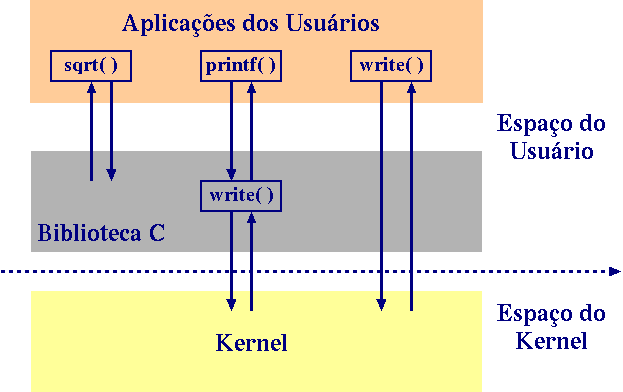
\includegraphics[width=0.6\textwidth]{assets/aula-tads-sopa2-2023-06-05/chamadas.png}}
            \caption{https://guialinux.uniriotec.br/chamadas-de-sistema/}
        \end{figure}
\end{frame}



\footlinecolor{}

\backmatter
\end{document}
